%=========================================================================
% (c) 2014, 2015 Josef Lusticky

\section{Networking}\label{sec:setup-networking}
Default installation of CentOS with the updates avaliable on 7th January 2015 installed,
including the distribution Linux kernel version 3.10.0-123.13.1.el7.x86\_64.


IPv4 addresses from 192.0.2.0/24 (TEST-NET-1) block were assigned~\cite{rfc5737}.
IPv6 addresses from 2001:db8::/32 range were assigned,
addresses within this block should not appear on the public Internet~\cite{rfc3849}.

Section%~\ref{}
described how the mlx4 drivers set up network interfaces.
In the measurements, IPv4 addresses 1.0.1.1 and 1.0.2.1 with 24-bit subnet mask were assigned to the interfaces.
%These subnets are not part of the BGP routes.
On the Spirent, the corresponding addresses 1.0.1.2 and 1.0.2.2 with 24-bit subnet mask were assigned.
Figure~\ref{fig:measurements-setup} shows the network scheme used for the measurements.
\begin{figure}[H]
	\centering
	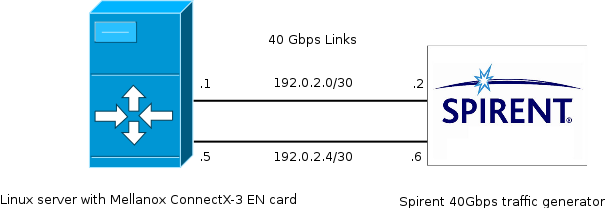
\includegraphics[width=13.5cm,keepaspectratio]{fig/net-setup.png}
	\caption{Measurement setup}
	\label{fig:measurements-setup}
\end{figure}


Enable IPv4 packet forwarding:
echo 1 > /proc/sys/net/ipv4/ip\_forward


ip neigh add 1.0.0.2 lladdr f4:52:14:5e:6c:71 dev enp6s0d1
ip neigh add 2.0.0.2 lladdr f4:52:14:5e:6c:70 dev enp6s0

ip addr add 1.0.0.1/24 broadcast 1.0.0.255 dev enp6s0d1
ip addr add 2.0.0.1/24 broadcast 2.0.0.255 dev enp6s0


Load BGP routes:
\begin{lstlisting}
Basic info: size of leaf: 40 bytes, size of tnode: 40 bytes.
Main:
        Aver depth:     2.43
        Max depth:      8
        Leaves:         503308
        Prefixes:       538739
        Internal nodes: 114430
          1: 58725  2: 26171  3: 14808  4: 7316  5: 4239  6: 2103  7: 1065  8: 2  17: 1
        Pointers: 995798
Null ptrs: 378061
Total size: 61373  kB
\end{lstlisting}
